\documentclass{article}
\usepackage{graphicx}
\usepackage{wrapfig}
\usepackage{xcolor}
\usepackage{amsmath}
\usepackage{verbatim}
\usepackage{makeidx}
\usepackage{float}
\usepackage{subfig}
\usepackage[left=1in,top=1in,right=1in]{geometry}

\title{Simulating the Mobot and Linkbot}
\author{Kevin Gucwa\\Mechanical and Aerospace Engineering}
\date{\today}
\makeindex

\begin{document}

\begin{center}
{\Huge\sf\bf RoboSim User's Guide}\\
\vspace*{2.5cm}
{\Large\bf Version 1.6.70}
\vspace{4in}

Copyright \copyright\ \today\ by UC Davis C-STEM Center, All rights reserved.

\end{center}

%\maketitle
\newpage
\tableofcontents
\newpage

\section{Introduction}
\texttt{RoboSim} is a robot simulation environment, developed by the UC Davis
Center for Integrated Computing and STEM Education (C-STEM) {\color{blue} \bf
(http://c-stem.ucdavis.edu)}, for programming Barobo Mobot and Linkbot.  The
same Ch program  can control hardware robots or virtual robots in RoboSim
without any modification.

\section{RoboSim GUI}
\label{sec:gui}
RoboSim can be conveniently launched by double clicking its icon

\includegraphics[height=24pt]{images/robosim} on the desktop.  The RoboSim
graphical user interface (GUI), shown in Figure \ref{fig:gui}, allows the user
to change between hardware and virtual robots when a Ch robot program is
executed.  There is no save button within the GUI, all changes made are
automatically saved.
\begin{figure}[H]
	\begin{center}
		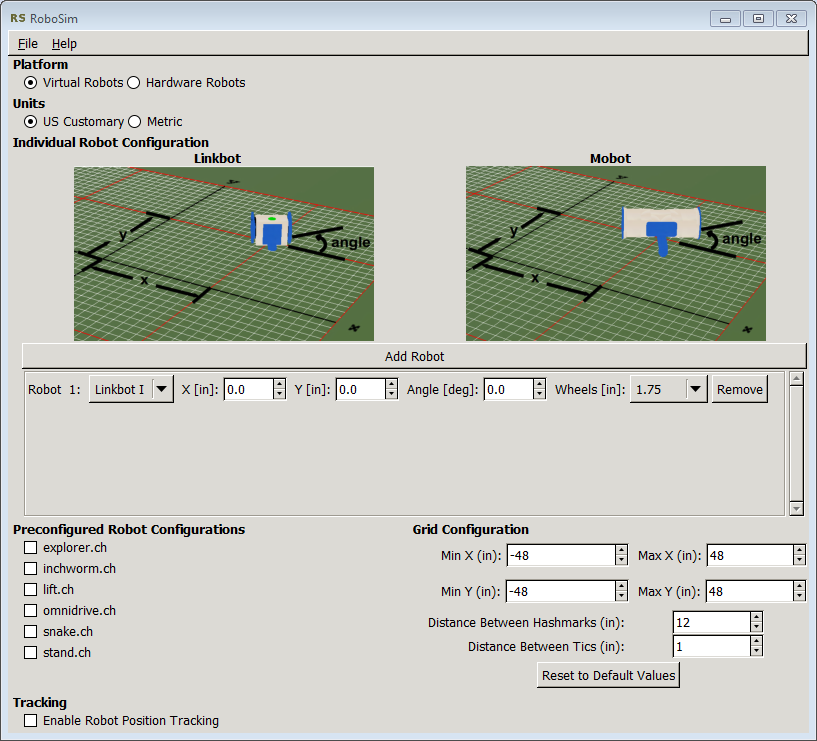
\includegraphics[width=6in]{images/gui}
	\end{center}
	\caption{The RoboSim GUI.}
	\label{fig:gui}
\end{figure}

\subsection{Platform}
The {\bf Platform} entry as shown in Figure \ref{fig:platform}, allows the user
to decide whether a Ch program controls the hardware or virtual robots.  Each
time a new Ch program is started, it will check the setup based on this entry.
For a Ch robot program to control a virtual robot, check the box for {\bf
Simulated Robots}.  If the box for {\bf Hardware Robots} is checked, a Ch
program will control the physical hardware robots.
\begin{figure}[H]
	\begin{center}
		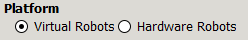
\includegraphics[width=3in]{images/gui_platform}
	\end{center}
	\caption{Initial robot configuration dialog.}
	\label{fig:platform}
\end{figure}

\subsection{Units}
\label{sec:units}
Simulations within RoboSim can be run either in {\bf US Customary} units
consisting of inches, degrees, and seconds or {\bf Metric} units with
centimeters, degrees, and seconds.  Changing units will effect the grid spacing
drawn beneath the robots and the spacing between robots.  Changing between these
two options will change the labels within the GUI to indicate the units being
used.

\subsection{Tracing}
{\bf Tracing} where robots have been can be enabled by selecting the check box
'Enable Robot Position Tracing', as shown in Figure \ref{fig:gui}.  When the
tracing is enabled, lines following the robot trajectories will be drawn for
each robot.  Mobot tracking lines will be in a green color and Linkbot tracking
lines will be in the color matching the Linkbot LED.

\subsection{Grid Configuration}
To be able to see how far robots have moved, a grid is enabled under the robots.
There are six options to alter the layout of the grid lines under the {\bf Grid
Configuration}.  The minimum and maximum extends of the grid for both the X and
Y directions can be specified individually.  Rectangular grids of any size can
be created in any of the quadrants.  Hashmarks are the red lines drawn within
the configuration images.  By default, the distance between two hashmarks is 12
inches in US Customary units and 50 centimeters in Metric units.  Tics are the
most frequent lines drawn in a light gray.  By default, the distance between two
tics is 1 inch in US Customary units and 5 centimeters in Metric units.

Switching between US Customary and Metric units will change these default values
to logical starting points for the metric system.  The 'Reset to Defaults' button
will allow the default values for both US Customary and Metric to be reinstated
after they have been changed.  Depending upon which units are currently selected
from Section \ref{sec:units}, either the US Customary defaults, shown in Figure
\ref{fig:grid_us}, or the Metric defaults, as shown in Figure
\ref{fig:grid_metric}, will be set.
\begin{figure}[H]
	\begin{center}
		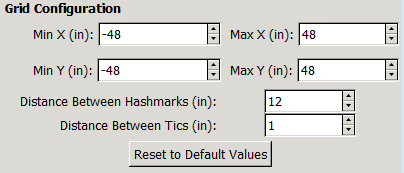
\includegraphics[width=4in]{images/gui_grid_us}
	\end{center}
	\caption{Default US Customary Grid Spacing.}
	\label{fig:grid_us}
\end{figure}
\begin{figure}[H]
	\begin{center}
		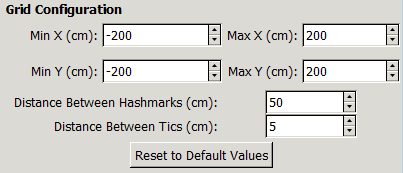
\includegraphics[width=4in]{images/gui_grid_si}
	\end{center}
	\caption{Default Metric Grid Spacing.}
	\label{fig:grid_metric}
\end{figure}

\subsection{Individual Robot Configuration}
Initial robot configurations can either be done through the {\bf Individual
Robot Configuration} or {\bf Preconfigured Robot Configuration} tabs.  The
{\bf Individual Robot Configuration} section, as shown in Figure
\ref{fig:config}, has options to allow robots to be positioned within the
RoboSim scene either with or without wheels but not attached to each other.
\begin{figure}[H]
	\begin{center}
		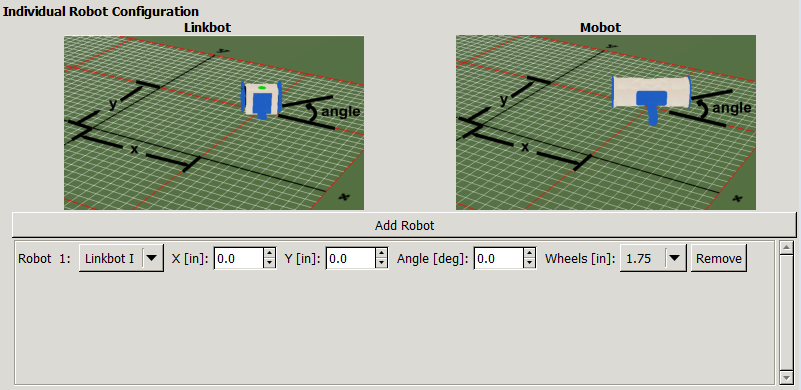
\includegraphics[width=6in]{images/gui_individual}
	\end{center}
	\caption{Individual robot configuration dialog.}
	\label{fig:config}
\end{figure}

The user can specify the X and Y coordinates  as well as the orientation angle
of a virtual robot.  Images for the Linkbot and Mobot showing the meaning of
each of the options are displayed above the configuration box.  They are
screenshots of the virtual robots positioned at one foot in both the X and Y
coordinates with the orientation angle of 30 degrees from the X-axis.

Initially, the individual robot list contains one Linkbot-I at (0, 0) with 1.75
inch wheels.  More robots can be added by the 'Add Robot' button.  Clicking this
button will add a robot into RoboSim, each offset from the previous one in the
x-direction by 6 inches or 15 centimeters depending upon the units selected.
The order within the robot list will be the order in which the robots will be
read into the simulation program.

\subsubsection{Robot Type}
There are three options for robot type available.  Linkbot-I, Linkbot-L,
and Mobot.  The options are presented in a drop down menu.
\begin{figure}[H]
	\begin{center}
		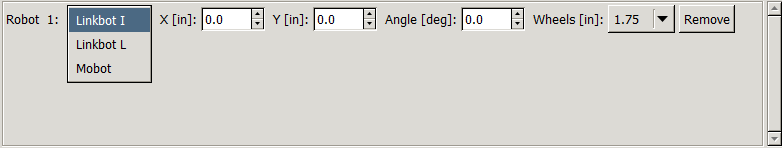
\includegraphics[width=6in]{images/gui_type}
	\end{center}
	\caption{Picking a robot type.}
	\label{fig:type}
\end{figure}

\subsubsection{Robot Position}
Both X and Y positions can be chosen independently for each robot.

\subsubsection{Robot Angle}
The rotation angle from the x-axis can be used for changing the orientation of
the two robots respective to each other.

\subsubsection{Wheels}
Since so many times the robots are run with wheels and a caster connected, a
drop down menu is provided to select different wheel sizes.  The options listed
are the radii of the wheels provided with Linkbots when purchased from Barobo.
Each wheel is drawn with a series of dots along the one radius to easily show
the rotation of the wheel.  The correlation between wheel radius and number of
dots is given in Table \ref{tab:wheels}.
\begin{table}[H]
	\begin{center}
	\begin{tabular}{c | l }
		\hline \hline
		\textbf{Number of Dots} & \textbf{Wheel Radius} \\ \hline
		2 & custom radius \\
		3 & 1.625 inch / 4.13 centimeter \\
		4 & 1.75 inch / 4.45 centimeter \\
		5 & 2.00 inch / 5.08 centimeter \\
		\hline \hline
	\end{tabular}
	\caption{Wheel sizes and number of dots.}
	\label{tab:wheels}
	\end{center}
\end{table}

Custom wheel sizes are available by using the 'Custom' option from the drop down
menu.  This option creates an input box to the right to let the user enter a
wheel radius.

\subsubsection{Remove}
A robot can be removed from the RoboSim by clicking the 'Remove' button.

\subsection{Preconfigured Robot Configurations}
In addition to positioning robots independently within the RoboSim, some {\bf
Preconfigured Robot Configurations}, as shown in Figure \ref{fig:preconfig},
which represent commonly used Linkbot configurations  are available to the user.
Selecting one of these options will display a picture of the configuration built
with the hardware Linkbots and corresponding to a Ch robot program presented in
Chapter 13 in the book {\em Learning Robot Programming with Linkbot for the
Absolute Beginner}.  When one of these options is selected, the specific
configuration for this setup is passed into Ch and robots specified in the
individual robot configuration are ignored.  To switch back to the individual
configuration, just unselect the selected preconfigured robot configuration.
\begin{figure}[H]
	\begin{center}
		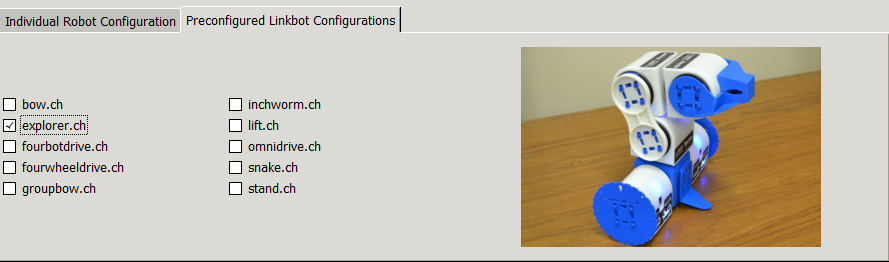
\includegraphics[width=6in]{images/gui_preconfig}
	\end{center}
	\caption{Preconfigured Linkbots.}
	\label{fig:preconfig}
\end{figure}

\section{Running a Ch Program with RoboSim}
Once the simulation environment has been configured with the RoboSim GUI in
Section \ref{sec:gui}, the user can run Ch programs in ChIDE to control the
virtual robots.  The RoboSim GUI should remain open while simulating robots.
Once it is closed, the system will revert to hardware mode.  The RoboSim scene
with virtual robots for each simulation are created upon running a Ch program.
For example, when the Ch program {\tt moveforward3.ch} below
\begin{verbatim}
/* File: moveforward3.ch
   Move forward for Linkbot-I as a two-wheel vehicle */
#include <linkbot.h>
CLinkbotI robot;

/* connect to the paired robot and move to the zero position */
robot.connect();
robot.resetToZero();

/* move forward by rolling two wheels for 360 degrees */
robot.moveForward(360);
\end{verbatim}
\noindent
is executed in ChIDE, a RoboSim scene shown in Figure \ref{fig:robosim_scene}
will be displayed.
\begin{verbatim}
    Paused: Press any key to start
\end{verbatim}
is displayed in the RoboSim scene to reminder the user that the virtual robot
will not move until the user presses any key on the keyboard. This gives the
user an opportunity to examine the RoboSim scene before the motion begins.
\begin{figure}[H]
	\begin{center}
		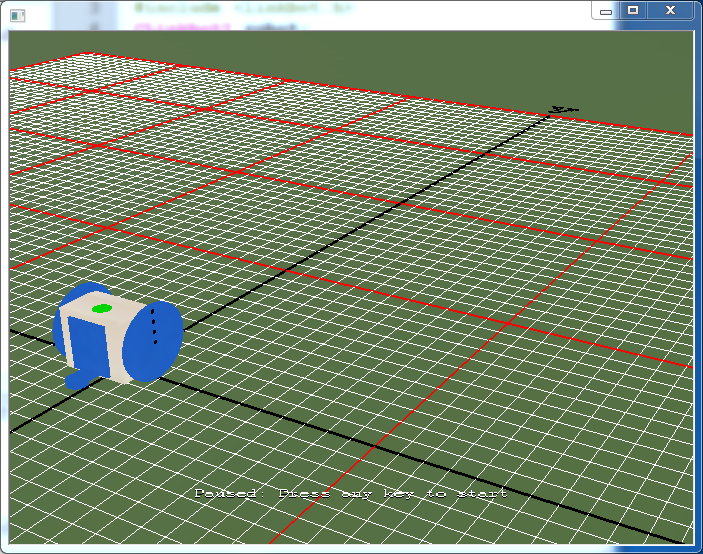
\includegraphics[width=3in]{images/robosim_scene}
	\end{center}
	\caption{A RoboSim scene with a virtual robot at its starting position.}
	\label{fig:robosim_scene}
\end{figure}

While a robot is moving in the RoboSim scene, the user can press any key to
pause the motion of the robot.  When the motion is paused, the message
\begin{verbatim}
    Paused: Press any key to restart
\end{verbatim}
will be displayed in the RoboSim scene. The user can press any key to restart
the motion.

When the user presses the 't' key, the robot trajectory is tracked in a green
line in the RoboSim scene as shown in Figure \ref{fig:robosim_tracked}.
\begin{figure}[H]
	\begin{center}
		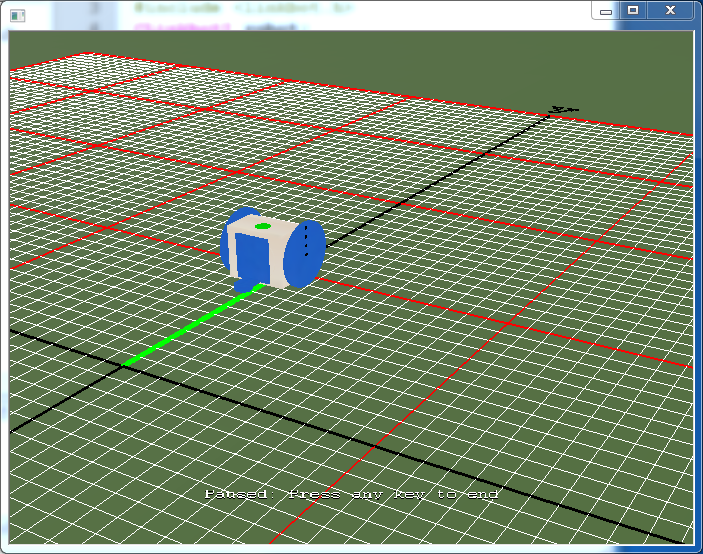
\includegraphics[width=3in]{images/robosim_tracked}
	\end{center}
	\caption{A RoboSim scene with a virtual robot and its trajectory tracked.}
	\label{fig:robosim_tracked}
\end{figure}

When the program is finished, the message
\begin{verbatim}
    Paused: Press any key to end
\end{verbatim}
will be displayed in the RoboSim scene.  Pressing any key, the RoboSim scene
will disappear.

\section{Interacting with a RoboSim Scene}
The user can interact with a RoboSim scene through the keyboard and mouse.

The ground plane is for reference only.  It is designed to disappear when
viewing the robots from below to be able to inspect the movement from all
angles.

\subsection{Keyboard Input}
The RoboSim scene responds to keyboard input as outlined in Table
\ref{tab:keys}.  As described in the previous sections,
the 't' key will toggle the tracking of robot trajectories.

\begin{table}[H]
	\begin{center}
	\begin{tabular}{c | l }
		\hline \hline
		\textbf{key} & \textbf{action} \\ \hline
		1 & return to home camera position \\
		2 & set camera to overhead view \\
		n & toggle grid line numbering \\
		r & toggle robot visibility and enable tracking \\
		t & toggle robot tracking \\
		any other key & Pause and unpause simulation \\
		\hline \hline
	\end{tabular}
	\caption{Keyboard input for RoboSim}
	\label{tab:keys}
	\end{center}
\end{table}

There are two views available to the user.  The default view, which can be
toggled with the '1' key, is from behind the robots looking into the first
quadrant.  This view can be seen in any of the RoboSim scene screenshots within
this document, except for Figure \ref{fig:robosim_overhead} which shows the
overhead view.  The '2' key moves the camera directly above the origin looking
down on the scene creating a 2D viewpoint of the robots.
\begin{figure}[H]
	\begin{center}
		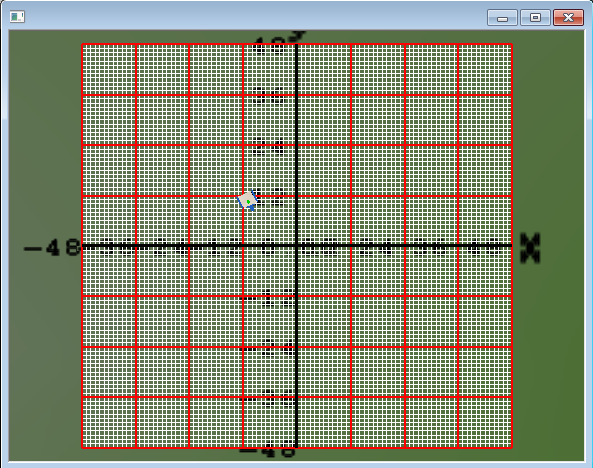
\includegraphics[width=3in]{images/robosim_overhead}
	\end{center}
	\caption{A RoboSim scene with the overhead viewing angle.}
	\label{fig:robosim_overhead}
\end{figure}

The 'n' key allows the user to toggle the display of the grid numbering.  X and
Y numbering is by default enabled and given for every hashmark on the grid.

The 'r' key will toggle the display of virtual robots or robot trajectories.
This feature is useful when the user would like to view a trajectory traced by a
robot without the virtual root blocking the trajectory.  Figure
\ref{fig:robosim_norobot} shows a RoboSim scene with a tracked robot trajectory
only.
\begin{figure}[H]
	\begin{center}
		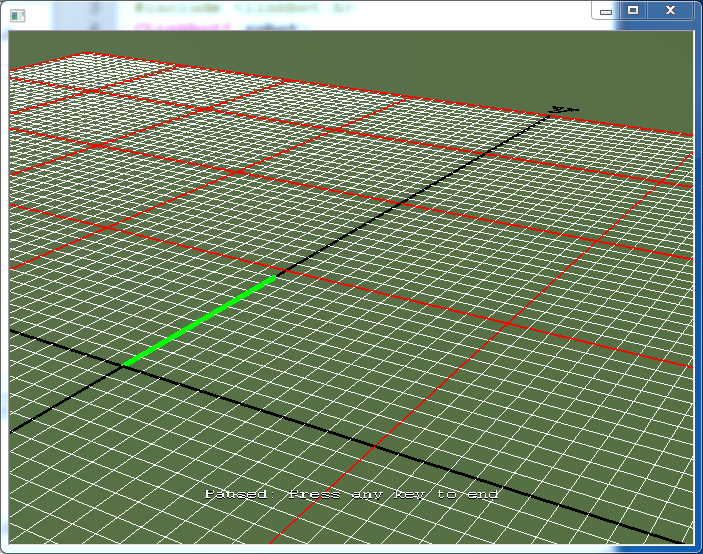
\includegraphics[width=3in]{images/robosim_norobot}
	\end{center}
	\caption{A RoboSim scene with a tracked robot trajectory only.}
	\label{fig:robosim_norobot}
\end{figure}

As described in the previous section, the motion of robots in the RoboSim scene
can be paused and restarted by pressing any other key on the keyboard.

\subsection{Mouse Input}
Clicking on a robot in a RoboSim scene will enable a pop up which displays the
robot number and the current position of the robot, as shown in Figure
\ref{fig:robosim_pos} with the position (0, 10.9817) inches for the X and Y
coordinates for the Robot 1.  Clicking again the displayed position for the
robot will disappear.
\begin{figure}[H]
	\begin{center}
		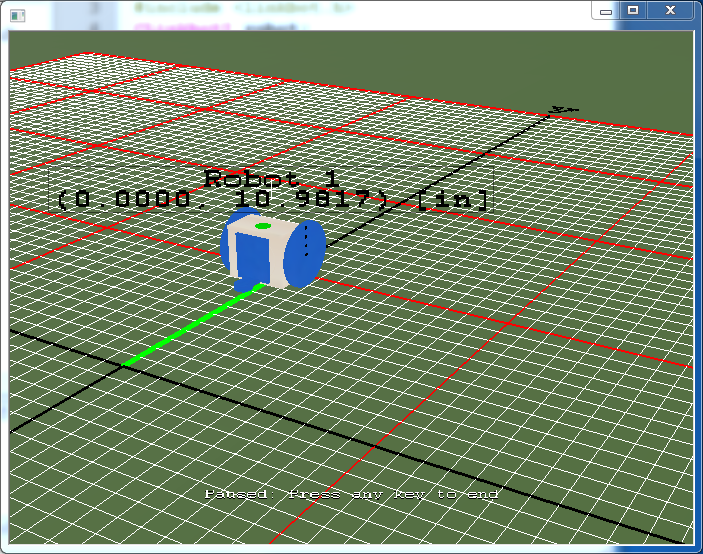
\includegraphics[width=3in]{images/robosim_pos}
	\end{center}
	\caption{A RoboSim scene with a virtual robot and its position displayed.}
	\label{fig:robosim_pos}
\end{figure}

The user can execute a Ch robot program in debug mode in ChIDE, line by line,
with the command {\tt Next}. At the end of each motion statement, the user can
click the robot in the RoboSim scene to obtain the X and Y coordinates of the
robot.  The ability to obtain the X and Y coordinates of a robot during its
motion along a trajectory can be very useful for learning many math concepts.

The mouse can be used to move the camera around the scene.  Holding the left
mouse button and dragging the mouse pans the camera as outlined in Table
\ref{tab:buttons}.  Holding the right mouse button and dragging the mouse
enables scaling of the view by zooming in and out.  Holding both left and right
mouse buttons and dragging changes the location of the camera within the scene.

The ground plane is for reference only.  The ground plane will disappear when
viewing the robots from below so that the user can inspect the movement from all
angles.

\begin{table}[H]
	\begin{center}
	\begin{tabular}{c | l }
		\hline \hline
		\textbf{button} & \textbf{action} \\ \hline
		Hold left mouse button and drag& rotate camera \\
		Hold right mouse button and drag& zoom in and out \\
		Hold both left and right buttons,  and drag & pan around scene \\
		Click on a robot & display the robot position\\
		\hline \hline
	\end{tabular}
	\caption{Mouse input for the RoboSim scene.}
	\label{tab:buttons}
	\end{center}
\end{table}

\section{Differences to Hardware}
RoboSim has some different options which affect the performance of the
simulation.  These are options which are passed into the connect function of the
robots that are not available within hardware.  The RoboSim GUI writes all of
the options into a user configuration file that has to be changed each time a
new code is to be run.  However, users can manually write configuration files
specific to each code.  To tell RoboSim to use a custom configuration file over
the global one, pass the name of the file into the first connect function call
in the file.  RoboSim will look in the same folder to find the configuration
file, if it is not found, then it will use the default one.
\begin{verbatim}
#include <linkbot.h>
CLinkbotI robot;

robot.connect("testrc");
\end{verbatim}




%% APPENDIX

\newpage
\appendix
\section{Manual Configuration File Generation}
All options available in the RoboSim GUI can be done manually as well as adding
in more advanced features which are not necessary to be exposed to all users in
the GUI.  There are four sections to the configuration file.  The header,
configuration, ground, and simulation sections.  Each holds specific types of
information about the simulation to be run.

\subsection{Header}
The header is one line and specifies to RoboSim that this is a valid xml file.
This line should be placed at the start of each simulation file.
\begin{verbatim}
<?xml version="1.0" encoding="UTF-8"?>
\end{verbatim}

\subsection{Configuration Section}
General parameters about the simulation can be added within the config section.
Each one is its own line placed between the starting \verb%<config>% and ending
\verb%</config>%.
\begin{verbatim}
<config>
</config>
\end{verbatim}

\subsubsection{Version}
\begin{verbatim}
<version val="1"/>
\end{verbatim}
The version of the XML configuration file.  Updated internally when new
non-backwards compatible changes are made.

\subsubsection{Type}
\begin{verbatim}
<type val="0"/>
\end{verbatim}
There are two options: either preconfigured robots or individual robots.  Used
to load the right options when launching the GUI.  Can be 0 to show that the
robots within the \verb%<sim></sim>% are individual.  Any number above that
represents the preconfigured robots within the GUI.

\subsubsection{Grid}
\begin{verbatim}
<grid units="1" major="12" tics="1" minx="-48" maxx="48" miny="-48" maxy="48"/>
\end{verbatim}
The grid boxes from the GUI put their information here.  \verb%units%: 1 for US
Customary and 0 for Metric.  \verb%major% are the red hashmarks and \verb%tics%
are the gray tick marks.  \verb%minx% and \verb%maxx% are the minimum and
maximum distances along the X-axis for the grids, respectively.  \verb%miny% and
\verb%maxy% are the complements for the Y-axis.

\subsubsection{Tracking}
\begin{verbatim}
<tracking val="1"/>
\end{verbatim}
Setting to track robot location with lines on the ground.  1 for on; 0 for off.

\subsubsection{Pause}
\begin{verbatim}
<pause val="1"/>
\end{verbatim}
The simulation can either start paused waiting for a user to press a key to
start or it will start as soon as it is ready.  Passing 0 to this option starts
the simulation; while 1 pauses it at the beginning.

\subsubsection{Real Time}
\begin{verbatim}
<realtime val="1"/>
\end{verbatim}
The simulation can run faster than real time.  Passing 0 to this option allows
the simulation to run as fast as the computer can simulate it.

\subsubsection{Mu}
\begin{verbatim}
<mu ground="0.9" body="0.3"/>
\end{verbatim}
The coefficient of friction can be altered between the robots and the ground and
between robots themselves.  The default values are given here.

\subsubsection{Coefficient of Restitution}
\begin{verbatim}
<cor ground="0.3" body="0.3"/>
\end{verbatim}
The coefficient of restitution can be altered between the robots and the ground
and between robots themselves.  The default values are given here.  The COR is a
measure of how bouncy a surface is.  Small values correspond to hard surfaces
while larger values are for softer surfaces.

\subsection{Ground Section}
The ground section holds the solid bodies which are a part of the ground for
which the robots to interact.  The objects do not need to be on the ground
plane.  They can be floating in space but are still a part of the ground
objects.  Everything to be added is put between the \verb%<ground>% tags.
\begin{verbatim}
<ground>
</ground>
\end{verbatim}

\subsubsection{Box}
\begin{verbatim}
<box>
    <size x="1" y="1" z="1"/>
    <position x="1" y="1" z="1"/>
    <rotation psi="1" theta="1" phi="1"/>
</box>
\end{verbatim}
The ground box is configured with the size, position, and rotation parameters.
The size gives the lengths in the X, Y, and Z directions.  Position gives the X,
Y, and Z location of the center of the box.  The rotation gives the three Euler
Angles of the box.

\subsubsection{Cylinder}
\begin{verbatim}
<cylinder>
    <size radius="1" length="10"/>
    <position x="1" y="1" z="1"/>
    <rotation psi="1" theta="1" phi="1"/>
</cylinder>
\end{verbatim}
The ground cylinder is configured with the size, position, and rotation
parameters.  The size gives the radius and length of the cylinder.  By default
the cylinder is drawn with the long axis along the X-axis.  Position gives the
X, Y, and Z location of the center of the cylinder.  The rotation gives the
three Euler Angles.

\subsubsection{Sphere}
\begin{verbatim}
<sphere>
    <size radius="1"/>
    <position x="1" y="1" z="1"/>
</sphere>
\end{verbatim}
The ground sphere is configured with the size and position parameters.  The size
gives the radius of the sphere.  By default the cylinder is drawn with the long
axis along the X-axis.  Position gives the X, Y, and Z location of the center of
the sphere.

\subsection{Simulation Section}
The simulation section holds the robots and accessories for the current
simulation.  Everything to be added is put between the \verb%<sim>% tags.
\begin{verbatim}
<sim>
</sim>
\end{verbatim}

\subsubsection{Robots}
Each robot has its own xml tag to configure its position, orientation, and
rotation in space.  The types of robot tags are tabulated in \ref{tab:robots}.
All robots much have attributes associated with them, and optionally positioning
arguments.  The Linkbot-T is a Linkbot with all three joints being able to
actuate.

\begin{table}[H]
	\begin{center}
	\begin{tabular}{c}
		\hline \hline
		\verb|<linkboti/>| \\
		\verb|<linkbotl/>| \\
		\verb|<linkbott/>| \\
		\verb|<mobot/>| \\
		\hline \hline
	\end{tabular}
	\caption{Robots}
	\label{tab:robots}
	\end{center}
\end{table}

\noindent
\newline
\textbf{Robot Attributes}
\newline
Each robot element is required to have one attribute titled \textbf{id} which is
an unique identifier for the simulation to reference.  A second optional
attribute is \textbf{orientation} which orients the face of a second robot when
it is being attached to a first robot.  A third optional argument is
\textbf{ground} which specifies which body part of the robot is attached to the
ground.  A fixed, permanent joint is created between this body part and the
ground.

\begin{table}[H]
	\begin{center}
	\begin{tabular}{c | l}
		\hline \hline
		\verb|<linkboti id="0"/>| & one Linkbot I with id = 0 \\
		\verb|<linkboti id="0" orientation="3"/>| & Linkbot I is 'upside-down' \\
		\verb|<linkboti id="0" ground="3"/>| & Linkbot I's face 3 is fixed \\
		\hline \hline
	\end{tabular}
	\caption{Examples}
	\label{tab:ex}
	\end{center}
\end{table}

\begin{table}[H]
	\begin{center}
	\begin{tabular}{c | c | l}
		\hline \hline
		\textbf{attribute} & \textbf{values} & \textbf{description} \\ \hline
		id & unique integer & a unique integer to identify each robot \\
		orientation & 1 & robot face number is at 12 o'clock \\
		 & 2 & robot face number is at 3 o'clock \\
		 & 3 & robot face number is at 6 o'clock \\
		 & 4 & robot face number is at 9 o'clock \\
		ground & 0 & body is attached to ground \\
		 & 1 & face 1 is attached to ground \\
		 & 2 & face 2 is attached to ground \\
		 & 3 & face 3 is attached to ground \\
		\hline \hline
	\end{tabular}
	\caption{Robot Attributes}
	\label{tab:attributes}
	\end{center}
\end{table}

\noindent
\newline
\textbf{Robot Positioning}
\newline
In addition to IDing each robot, they can be positioned in space independently
of each other.  There are sub-tags which specify the global attributes of
the robot.  \verb%<position>% specifies the X, Y, and Z coordinates of the
robot.  \verb%<rotation>% specifies the three Euler Angles of the robot about
the X (psi), Y (theta), and Z (phi) axes.  \verb%joint% allows the joints to be
rotated initially as opposed to being built at zero rotation.  Examples of
Linkbot and Mobot are shown below.
\begin{verbatim}
<linkboti id="0">
    <position x="0" y="0" z="0"/>
    <rotation psi="0" theta="0" phi="0"/>
    <joint f1="-20" f2="0" f3="20"/>
</linkboti>
\end{verbatim}
\begin{verbatim}
<mobot id="0">
    <position x="0" y="0" z="0"/>
    <rotation psi="0" theta="0" phi="0"/>
    <joint a1="-20" a2="0" a3="20" a4="45"/>
</mobot>
\end{verbatim}

\noindent
\newline
\textbf{Attaching Robots}
\newline
When a second robot is going to be attached to the first robot, the only
required argument is the id number.  The positioning will be figured out
automatically.  The code below shows the configuration for the inchworm linkbot
configuration.  The first robot is placed at the origin and the second one is
positioned by the code since it is attached to the bridge connector to the first
one.
\begin{verbatim}
<linkbotl id="0">
    <position x="0" y="0" z="0"/>
    <rotation psi="0" theta="180" phi="0"/>
</linkbotl>
<linkbotl id="1"/>
<bridge>
    <side id="1" robot="0" face="1"/>
    <side id="2" robot="1" face="1"/>
</bridge>
\end{verbatim}

All robots have faces onto which accessories can connect.  These are the points
of reference on how the robot will be positioned in space when attaching to
another robot.  The Mobot has eight connection faces, as shown in Figure
\ref{fig:mobot_connections}.  Faces 3 and 6 span the two body joints and thus
provide a physical connection which prevents the Mobot from bending its body.
The three Linkbot faces, shown in Figure \ref{fig:linkbot_connections}, are on
each of the three sides of the robot.  Two will be attached to the rotating
faces of the robot depending upon whether the robot is a Linkbot-I or a
Linkbot-L.
\begin{figure}[H]
	\begin{center}
		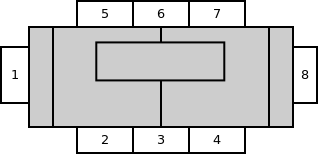
\includegraphics[width=3in]{images/mobot_connections}
	\end{center}
	\caption{Mobot Connection Locations.}
	\label{fig:mobot_connections}
\end{figure}
\begin{figure}[H]
	\begin{center}
		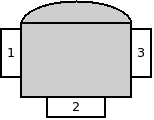
\includegraphics[width=2in]{images/linkbot_connections}
	\end{center}
	\caption{Linkbot Connection Locations.}
	\label{fig:linkbot_connections}
\end{figure}

\subsubsection{Accessories}
The accessories of the robots can be added to the scene and attached to the
robots by the tags.  Most accessories have multiple sides which are each
configured independently.  The options for a side are its id, robot which is
attached to that side, and the face of that robot.
\begin{verbatim}
<side id="1" robot="1" face="1"/>
\end{verbatim}

All sides are options which reside under the main accessory tag.  The
accessories available are shown in Table \ref{tab:acc}.

\begin{table}[H]
	\begin{center}
	\begin{tabular}{c | c | c | l}
		\hline \hline
		\textbf{Number} & \textbf{Accessory} & \textbf{Num. of Sides} & \textbf{Robot} \\ \hline
		0 & bigwheel & 1 & both \\
		1 & bridge & 2 & linkbot \\
		2 & caster & 1 & both \\
		3 & cube & 5 & linkbot \\
		4 & faceplate & 1 & linkbot \\
		5 & gripper & 1 & linkbot \\
		6 & l & 3 & mobot \\
		7 & omnidrive & 4 & linkbot \\
		8 & simple & 2 & both \\
		9 & smallwheel & 1 & both \\
		10 & square & 4 & mobot \\
		11 & tank & 3 & mobot \\
		12 & tinywheel & 1 & linkbot \\
		13 & wheel & 1 & both \\
		\hline \hline
	\end{tabular}
	\caption{Robot Accessories}
	\label{tab:acc}
	\end{center}
\end{table}

\noindent
\newline
\textbf{Multiple Sided Accessories}
\newline
Accessories with multiple sides are configured with that number of
\verb%<side/>% tags as shown in this bridge example.
\begin{verbatim}
<bridge>
    <side id="1" robot="0" face="1"/>
    <side id="2" robot="1" face="3"/>
</bridge>
\end{verbatim}

This will connect a bridge between robots with ids 0 and 1 on the robot's faces
1 and 3, respectively.

\noindent
\newline
\textbf{One-Sided Accessories}
\newline
Accessories with only one side are configured with the robot and face options
within the robot tag as shown in the wheel example below.
\begin{verbatim}
<smallwheel robot="1" face="3"/>
\end{verbatim}

\noindent
\newline
\textbf{Daisy-Chaining}
\newline
Since accessories of the Linkbot can be attached to each other and not just
directly to the robot, there are options to daisy-chain the accessories
together.  To do this, the \verb%face% option is replaced for a side with the
\verb%conn% option and the number corresponding to the accessory shown in the
first column of Table \ref{tab:acc}.  The example below shows the simple
connector with a smallwheel attached to the third face of the robot.
\begin{verbatim}
<simple>
    <side id="1" robot="0" face="3"/>
    <side id="2" robot="0" conn="9"/>
</simple>
\end{verbatim}

\noindent
\newline
\textbf{Custom Wheel Sizes}
\newline
Custom wheel radii can be entered into the configuration file when using the
\verb%wheel% option.  The radii of the preconfigured big, small, and tiny wheels
are set internally to correspond to the produced wheels.  Inputting a custom
wheel radius is done through the \verb%side% option when daisy-chaining a wheel.
Below is a daisy-chained custom wheel with a radius of 0.001 meters.
\begin{verbatim}
<simple>
    <side id="1" robot="0" face="1"/>
    <side id="2" robot="0" conn="13" radius="0.001"/>
</simple>
\end{verbatim}

\subsection{Examples}
Some example configuration files.

\subsubsection{One Robot at (0, 0, 0)}
\begin{verbatim}
<?xml version="1.0" encoding="UTF-8"?>
<config>
    <version val="1"/>
    <type val="0"/>
	<grid units="1" major="12" tics="1" minx="-48" maxx="48" miny="-48" maxy="48"/>
    <tracking val="1"/>
</config>

<sim>
    <linkboti id="0">
        <position x="0" y="0" z="0"/>
        <rotation psi="0" theta="0" phi="0"/>
    </linkboti>
    <simple>
        <side id="1" robot="0" face="1"/>
        <side id="2" robot="0" conn="9"/>
    </simple>
    <simple>
        <side id="1" robot="0" face="3"/>
        <side id="2" robot="0" conn="9"/>
    </simple>
    <caster robot="0" face="2"/>
</sim>
\end{verbatim}

\subsubsection{Two Robots on X-Axis}
\begin{verbatim}
<?xml version="1.0" encoding="UTF-8"?>
<config>
    <version val="1"/>
    <type val="0"/>
	<grid units="1" major="12" tics="1" minx="-48" maxx="48" miny="-48" maxy="48"/>
    <tracking val="1"/>
</config>

<sim>
    <linkboti id="0">
        <position x="0" y="0" z="0"/>
        <rotation psi="0" theta="0" phi="0"/>
    </linkboti>
    <simple>
        <side id="1" robot="0" face="1"/>
        <side id="2" robot="0" conn="9"/>
    </simple>
    <simple>
        <side id="1" robot="0" face="3"/>
        <side id="2" robot="0" conn="9"/>
    </simple>
    <caster robot="0" face="2"/>
    <linkboti id="1">
        <position x="0.1524" y="0" z="0"/>
        <rotation psi="0" theta="0" phi="0"/>
    </linkboti>
    <simple>
        <side id="1" robot="1" face="1"/>
        <side id="2" robot="1" conn="9"/>
    </simple>
    <simple>
        <side id="1" robot="1" face="3"/>
        <side id="2" robot="1" conn="9"/>
    </simple>
    <caster robot="1" face="2"/>
</sim>
\end{verbatim}

\subsubsection{Explorer}
\begin{verbatim}
<?xml version="1.0" encoding="UTF-8"?>
<config>
    <version val="1"/>
    <type val="1"/>
	<grid units="1" major="12" tics="1" minx="-48" maxx="48" miny="-48" maxy="48"/>
    <tracking val="1"/>
</config>

<sim>
    <linkboti id="0">
        <position x="0" y="0" z="0"/>
        <rotation psi="0" theta="0" phi="-90"/>
    </linkboti>
    <linkboti id="1"/>
    <linkboti id="2" orientation="3">
        <joint f1="-20" f2="0" f3="20"/>
    </linkboti>
    <linkboti id="3">
        <joint f1="-90" f2="0" f3="90"/>
    </linkboti>
    <linkbotl id="4" orientation="3"/>
    <simple>
        <side id="1" robot="0" face="3"/>
        <side id="2" robot="0" conn="9"/>
    </simple>
    <simple>
        <side id="1" robot="1" face="1"/>
        <side id="2" robot="1" conn="9"/>
    </simple>
    <cube>
        <side id="1" robot="0" face="1"/>
        <side id="2" robot="0" conn="2"/>
        <side id="3" robot="1" face="3"/>
        <side id="5" robot="2" face="2"/>
    </cube>
    <bridge>
        <side id="1" robot="2" face="1"/>
        <side id="2" robot="3" face="1"/>
    </bridge>
    <bridge>
        <side id="1" robot="2" face="3"/>
        <side id="2" robot="3" face="3"/>
    </bridge>
    <simple>
        <side id="1" robot="3" face="2"/>
        <side id="2" robot="4" face="2"/>
    </simple>
    <gripper robot="4"/>
</sim>
\end{verbatim}
\end{document}
